\documentclass{template/llncs} %geen idee wa dees is
%\documentclass[11pt,a4paper,oneside]{article}
\usepackage{makeidx}  % allows for indexgeneration
\usepackage{a4wide} %bredere tekst
\usepackage[english]{babel} % woorden juist afsplitsen
\usepackage{graphicx} %afbeeldingen ?
\usepackage[utf8]{inputenc}
\usepackage{textgreek}
\usepackage{url}
\usepackage{subcaption}
% Volgend package is niet echt nodig. Het laat echter toe om gemakkelijk elektronisch
% te navigeren in je pdf-document. Deze package moet altijd als laatste ingeladen worden.
\usepackage[a4paper,plainpages=false]{hyperref}    % Om hyperlinks te hebben in het pdfdocument.
\setlength{\parindent}{0cm}             % Inspringen van eerste lijn van paragrafen is niet gewenst.


%commando's
\newcommand{\npar}{\par \vspace{2.3ex plus 0.3ex minus 0.3ex}} %nieuwe paragraaf

\graphicspath{{images/}} %afbeeldingen in images zetten
\newcommand{\mijnfiguur}[4][h!]{            % Het eerste argument is standaar `ht'. op H zetten voor HIER EN NERGENS ANDERS
    \begin{figure}[#1]                      % Beginnen van de figure omgeving
        \begin{center}                      % Beginnen van de center omgeving
            \includegraphics[#2]{#3}        % Het eigenlijk invoegen van de figuur (2: opties, 3: bestandsnaam)
            \caption{#4\label{#3}}          % Het bijschrift (argument 4) en het label (argument 3)
        \end{center}
    \end{figure}
}

% make a proper TOC despite llncs
\setcounter{tocdepth}{3}
\makeatletter
\renewcommand*\l@author[2]{}
\renewcommand*\l@title[2]{}
\makeatletter

%%document zelf
\begin{document}
\frontmatter          % for the preliminaries
\pagestyle{headings}

\title{Project Image Processing}

\author{Andreas De Lille \and Cedric De Pauw \and Jo Van Damme  \and Kilian Hendrickx \and Patrick Van Staey}

\institute{Ghent University}
\date{}

\maketitle              % typeset the title of the contribution

\begin{abstract}
%\section{Abstract}

\npar
Navigating from place A to place B is not an easy task for blind or visually impaired people.
They heavily rely on memory and use tools such as a white cane, used to feel the road ahead.
Usually visually impaired people remember a list of steps by heart. When they use a route the go through the list one step at a time. Because of this, most of them only know 5 routes.
\npar
Because GPS signals have poor reception in dense populated areas, a combination of GPS and image processing is used. Both systems will work together to cancel out miscalcutations while providing a more reliable positioning system.
This project focusses on the image processing part. First the route is divided in smaller zones then each zone is characterized by a subset of features. These features are identified while a blind or visually impaired person follows his route,  and used to locate the blind person.
\npar
The goal of this project is not to make a realtime system, but to explore which features are useful.
Therefor the route from Sint-pietersstation in Ghent to Campus Schoonmeersen Ghent is selected as a training route. This route is divided in segments characterized by features that are recognized by a SVM (Support Vectoring Machine). The goal of this project is to prodive a script that, once given a movie, can analyse each frame and report the corresponding zone.
\npar
\clearpage
\end{abstract}%abstract & inleiding tesamen

\tableofcontents
\clearpage
\mainmatter
\section{Introduction}
Image processing creates a lot of potentionally groundbreaking developments, aiding visually impaired and blind people being one of them. Because these people have to learn each route by heart, most of them only know 5 routes. This has a large impact on their lifestyle and relatives. Image processing could offer a solution by assisting these people with navigation.
\npar
This project aims to create such a system by using image processing to assists blind or visually impaired persons. This system could then be used in combination with a GPS. The GPS would be used to determine the exact location, however when no GPS reception is available, the system would fall back on image processing to locate the person. Since the time for this project is limited, the goal is to create a script that classifies the zone for each frame from a given movie using only image processing. 
\npar
To acomplish this, the system must learn a route. This is done by dividing the route in zones, each characterized by their own unique combination of features. The first part of this project is the segmentation; division of the route in different zones. The seconds part will then select good recognizable features for extraction followed by mapping each unique subset of features on the corresponding zone. Once the features are extracted and mapped on zones a SVM is used to identify these features. The results of this SVM will provide the zone.
\npar
First up is an explaination about the SVM, the SVM used is \(SVM^{perf}\).
This is followed by a detailed explanation of features and the segmentation before the reports ends with the conclusion.

%werking svm? => ergens tussen steken
\clearpage
\section{SVM}
In machine learning, support vector machines (SVM) are supervised learning models with associated learning algorithms. They analyze data and recognize patterns used for classification and regression analysis. Given a set of training examples, each marked as belonging to one of two categories indicated by either -1 or +1.
\npar
An SVM training algorithm builds a model that assigns new examples into one category or the other, making it a non-probabilistic binary linear classifier. The more sure the algorithm is of its classification the more positive/negative the given value will be.
The closer the classification is to zero the more likely it is to get a false postive.
\npar
A SVM performs classification by constructing an N-dimensional hyperplane that optimally separates the data into two categories. An SVM model is a representation of the examples as points in space, mapped so that the examples of the separate categories are divided by a clear gap that is as wide as possible. New examples are then mapped into that same space and predicted to belong to a category based on which side of the gap they fall on.
\npar
The recommended SVM, \(SVM^{perf}\)\footnote{\url{http://www.cs.cornell.edu/people/tj/svm_light/svm_perf.html}}, was used for this application.
\(SVM^{perf}\) is an implementation of the Support Vector Machine (SVM) formulation for optimizing multivariate performance measures described in [Joachims, 2005].
\npar
As shown in Figures \ref{tree1} and \ref{tree2} several SVM's were used to create a tree structure to classify each frame to a zone.
\npar
The challenge with a SVM is finding the right training data for each feature. The right data is needed to make the Classification as correct as possible thus minimising the chance of a false positive. 

To optimize Accuracy, Precision en Recall:
\npar
TP = True Positive,
TN = True Negative,
FP = False Positive,
FN = False Negative
\npar
$Accuracy = (TP + TN) / (TP + TN + FP + FN)$

$Precision = TP / (TP+FP)$

$Recall = TP / (TP+FN)$

\mijnfiguur{width=0.5\textwidth}{svmtable}{SVM table}

in words

Accuracy = \% correct classified items.

Precision = \% selected items ( cat. +1) that are correct.

Recall = \% correct items that are selected.

\clearpage

%features => deze features worden gebruikt bij de zone
\section{Features}
\subsection{Grass}
\subsubsection{Idea} 
%Because grass keeps its green color during the year, it's a constant and reliable feature. % ni waar
Colordetection is a simple tool to detect grass, however a large variation in hue and saturation can cause problems.
Apart from the shadow and reflection, the colour of grass show lots of variations caused by external factors e.g. soil moisture, trash, seasons, weather. Therefore a large range of green must be considered as grass.
\npar
This section will discuss a few different approaches, each improving with the knowledge of the previous ones.
It is important to point out that in all of the approaches, the frame is converted from Blue Green Red (BGR)\footnote{BGR and RGB are equivalent colour spaces, except values are stored in a different order} \footnote{\url{http://infohost.nmt.edu/tcc/help/pubs/colortheory/web/color-wheel.html}} to Hue Saturation Value (HSV)\footnote{\url{http://infohost.nmt.edu/tcc/help/pubs/colortheory/web/hsv.html}}.
Since the person walks next to the grass rather than on it, grass is only found at the left or the right side.
\subsubsection{How it works}
To define the location if the grass is on the left or right side, the frame is cut in 3 parts. Only the left and right part are kept. Note that while the perspective of the image could be converted to bird's-eye-view, no problems where caused by skipping this step.
\paragraph{First approach}
To identify grass in a frame, an ideal colour of grass must be defined. This calibration took place by defining the average HSV values from a collection of pictures of grass. The result were these HSV values:
H: 60
S: 109
V: 94
\footnote{Note that H in OpenCV ranges between 0 and 180 instead of 0 and 360 and S and V range between 0 and 255 instead of 0 and 100.}
\npar
The left and right side of the image is cut in smaller parts, then the average colour of each part is calculated by
using the \(\sqrt{a^2 + b^2 + c^2}\) formula. The smallest value on each side gives the feature value. A small
values implies a small distance and therefor the presence of grass.  This causes a problem, since red is located both on the lower and upper side of the H space, while green is located in the center. the average of 2 red colors on each side of the H space will be centered and therefor green. This means that when a frame contains a lot of brown (which in its turn contains a lot of red) the average is located in the center and therefor also green. This is considered a bad average since the system now identifies both brown and green as grass.

\mijnfiguur{width=0.9\textwidth}{huered}{Red located at both edges of the H space, while green is found in the middle}

\clearpage
\subsubsection{Using a weight factor}
In an attempt to avoid these bad averages, the OpenCV function \(inRange()\)\footnote{\url{http://docs.opencv.org/modules/core/doc/operations_on_arrays.html\#inrange}} was used to preprocess the image. Colors in a centered range are kept before the average distance is calculated. However, because only green pixels are left in the selected image, the distance is always low even when one green pixel is found. A weight factor had to combine both results, however an ideal factor was never found. Since the average still contains a lot of false positives, a new method is needed.

\subsubsection{Third approach}
Since the bad averages are caused by red colors in the image, the second approach will calculate the fraction of red in the image. This calculation is, like the previous method, calculated by using the \(inRange()\) function. This time
however to select the red color instead of green. When this value is higher than 0.25, a penalty on the calculated
distance is given. The penalty is related to the fraction of green pixels in order to keep the distance of frames with
both red and green colors low . Also an additional penalty is given when the S component is low. A low S component
corresponds with graycolors and causing the H component to be less significant.
\npar
While the output of this classification looks promising, the SVM has trouble classifing the frames. Valid frames are in
the \(\left]0;70\right[\) interval, invalid in \(\left]80,140\right[\). This small margin appears to be too small for
the SVM.

\subsubsection{Final approach}
\npar
When developping the third approach, it became clear that only the selection of green pixels is reliable. Therefor only
the green pixels are used in this approach. All pixels matching \(H \in \left[29,45\right]\) \(S \in
\left[45,255\right]\) \(V \in \left[36,255\right]\) are counted and produce good results. This created a big difference
in valid and invalid frames, giving the SVM the posibility to classify the frames.

\subsubsection{Futher ideas}
\npar
Using the exact number of valid pixels in the SVM is a bad solution. When a different resolution is used, new training
is necessairy since the number of valid pixels could be much higher than before. An improvement would be to calculate
the fraction of green pixels over all pixels. This is more consistant with different resolutions.
By using only color to detect grass, other green objects are also identified. Texture might bring a solution but is hard to implement.
\clearpage
\subsection{Zebra crossing}
\label{zebrasection}
\subsubsection{Idea}
This feature will recognize a zebra crossing. The crossing is located outside the station before the blind person turns into the Sint-Denijslaan.
A zebra crossing consists of white rectangles with a certain size and shape, see Figure \ref{zebra}. However, these rectangles can be covered with dirt, making recognization difficult.
%\clearpage
\mijnfiguur{width=0.45\textwidth}{zebra}{A zebra crossing consists of white rectangles which can bo coverd with dirt}

\subsubsection{First approach}
The first approach uses a simple rectangle recognising system\footnote{This algoritm was found on github (\url{https://github.com/Itseez/opencv/blob/master/samples/cpp/squares.cpp})}.
Since the rectangle system was already used to determine the different tile sizes, the new algorithm would start from this system. With small modifications and calibrations, the program is able to find multiple rectangles. However since this approach ignores colors, found rectangles aren't always white. This created an unacceptable amount of false positives.
\npar
To solve this, the image is converted into a grayscale image. Then a small blur effect is applied to even out noise. After the noise-cancelling, the image is thresholded to create a mask. This mask is applied to the original image giving a remaining image that only has white colors, shown in Figure \ref{zebra2}.
\npar
\mijnfiguur{width=0.45\textwidth}{zebra2}{The white colors remain}
\clearpage
Since the system searches for white rectangles between a mininum and maximum size, results are improved. However false positives are still reported. To cancel out these false positives, a ratio is calculated and only rectangles whose ratio is between a lower and upper limit are allowed. This ratio enforces the shape of the rectangle while reducing false positives.
\npar
This version finds some rectangles, however if the duration of the crossing is 100 frames, only 5 frames are reported positive, this is unacceptable. Another downside is the processing time, the system that detects rectangles does mulitple iterations and searches for contours in every color dimension. This is quite useless since the image is converted to a grayscale. Then it is masked on the original image before it's handed over to the detector. Since the detector only uses one color dimension at a time, the image is again transformed. Masking and converting back and forth between colorspaces in combination with multiple iterations causes a lot of unnecessary overhead. The aforementioned problem calls for a new approach that uses less processing time and finds more white rectangles.

\subsubsection{Second approach}
The second approach will design a new findRectangle algoritm that doesn't rely on the existing one. This algoritm recieves a frame that is downsampled with the pyrDown function then upsampled with the pyrUp function to lower the noise. After that, the image is converted into a grayscale image and blurred. Then the white values are kept by thresholding the image. Once completed, the image is dilated. Both the dilation and blur effects are used to smooth the image\footnote{This is explained in a opencv tutorial found here: \url{http://docs.opencv.org/doc/tutorials/imgproc/gausian_median_blur_bilateral_filter/gausian_median_blur_bilateral_filter.html}} reducing the impact of the dirt shown in Figure \ref{zebra}. After the dilation the canny edge detection is used. Figure \ref{zebra_orig} shows the original frame while Figure \ref{zebrawitcanny} shows the edges found by the canny edge detection algorithm.
\begin{figure}[ht]
\centering
\caption{Comparison of a frame before and after the canny edge detection.}
\begin{subfigure}{.5\textwidth}
  \centering
  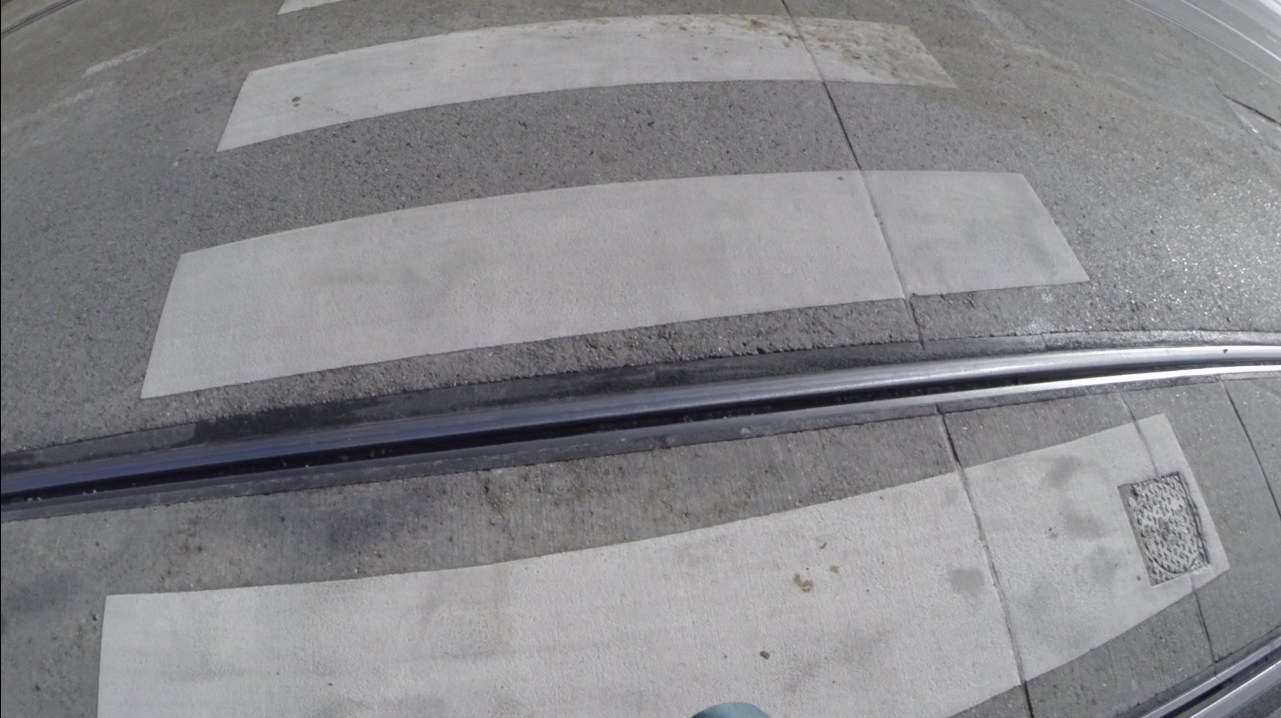
\includegraphics[width=.9\textwidth]{zebra_orig}
  \caption{Original frame\label{zebra_orig}}
\end{subfigure}%
\begin{subfigure}{.5\textwidth}
  \centering
  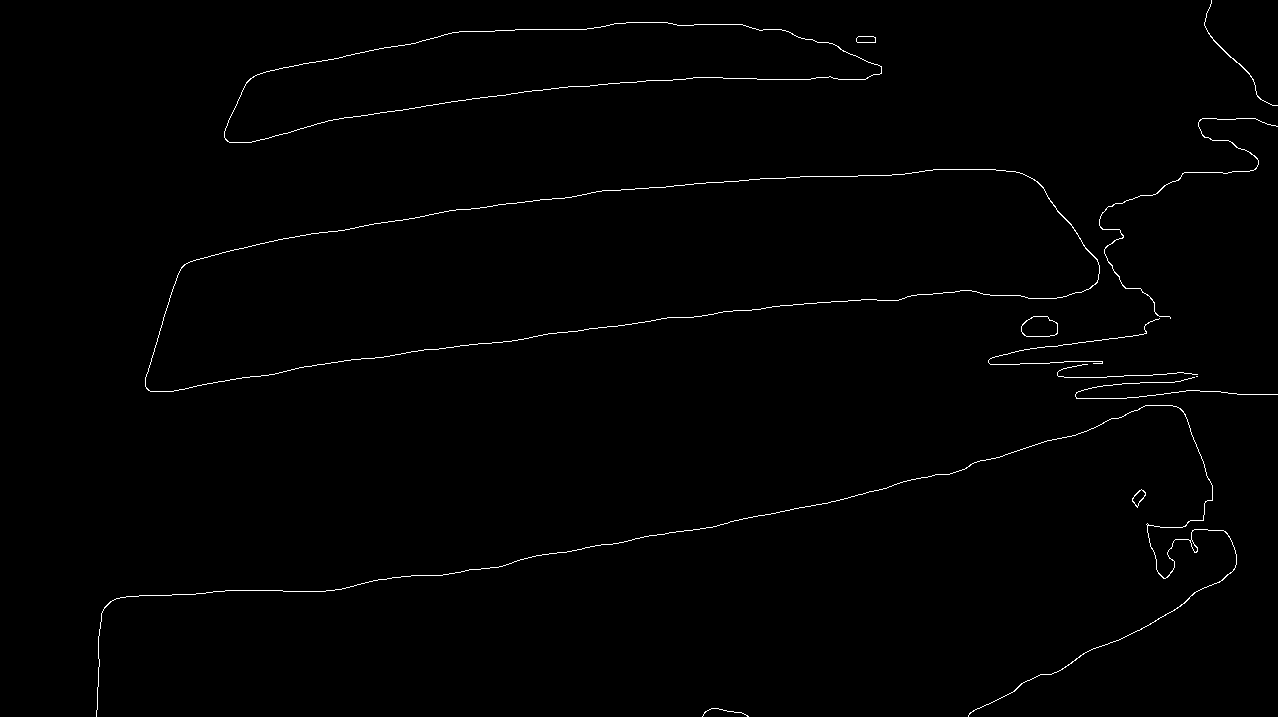
\includegraphics[width=.9\textwidth]{zebrawitcanny}
  \caption{After Canny\label{zebrawitcanny}}
\end{subfigure}
\end{figure}
\npar
Once the edges are found, the findContours function is used to find contours in the image\footnote{\url{http://docs.opencv.org/modules/imgproc/doc/structural_analysis_and_shape_descriptors.html?highlight=findcontours}}. The size and shape of each contour is tested using the ratio of the width / height.Also the size is measured. Since this function uses only one conversion and no iterations, the processing time is reduced approx to one-tenth of the original time.
\clearpage
However the second requirement of finding more rectangles isn't met. The cause of this problem is the high amount of dirt
on the white rectangles. Figure \ref{probvoor} shows the original image, Figure \ref{probna} shows the resulting canny
edge detection. It is clear that, in order to find a big rectangle in Figure \ref{probna}, the dirt must be removed. Note that not only dirt but also a shadow can cause this problem. Developping a solution for this problem takes time, so this feature isn't used for classification.
\begin{figure}[ht]
\centering
\caption{A frame showing a rectangle covered with dirt and its corresponding canny edge detection result.}
\begin{subfigure}{.5\textwidth}
  \centering
  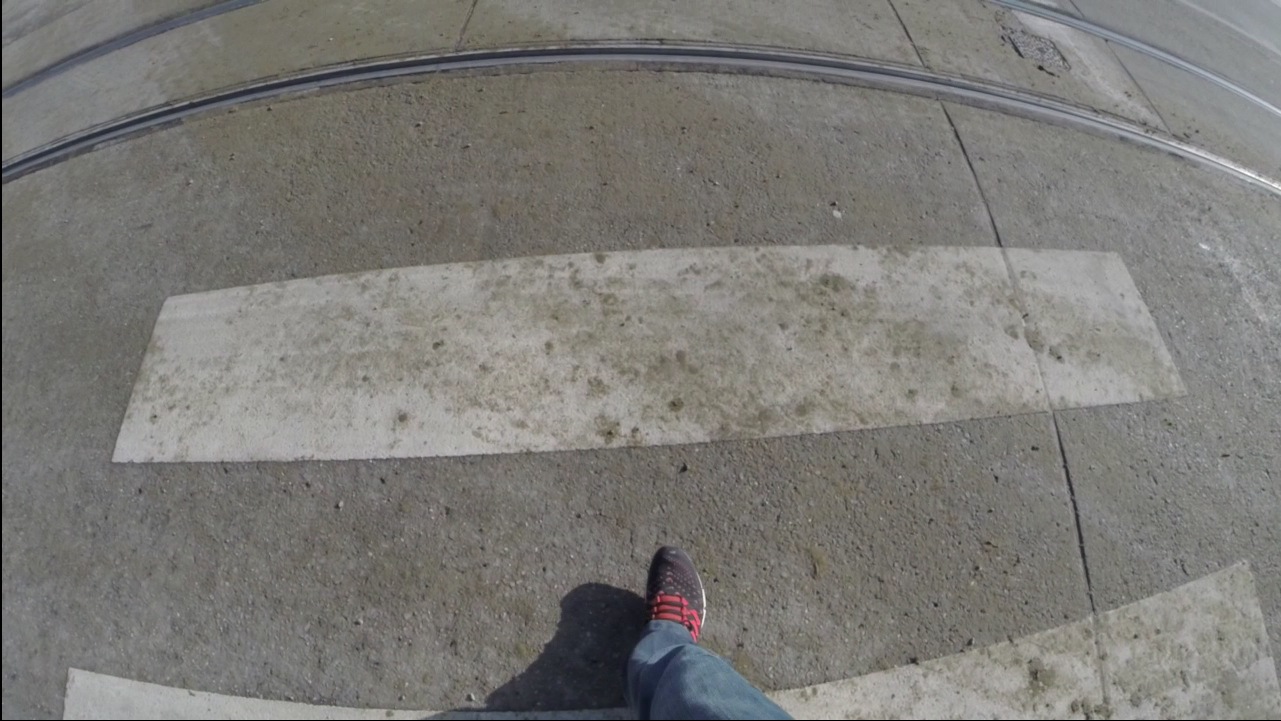
\includegraphics[width=.9\textwidth]{probvoor}
  \caption{Original frame\label{probvoor}}
\end{subfigure}%
\begin{subfigure}{.5\textwidth}
  \centering
  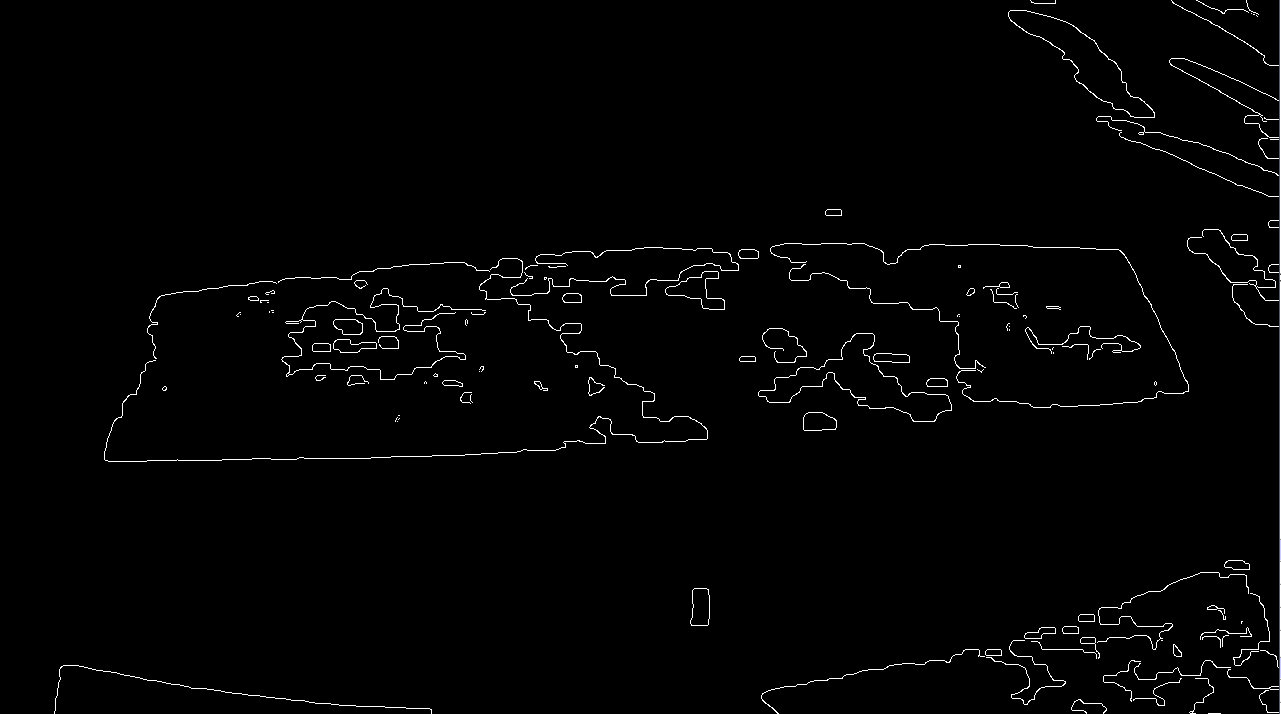
\includegraphics[width=.9\textwidth]{probna}
  \caption{\label{probna}}
\end{subfigure}
\end{figure}

\npar
When the dirt is on the edge of a rectangle, as shown in Figure \ref{dirtycorner}, the problem could be solved by ignore that edge. The edge detection won't find a rectangle but a trapezoid, shown in Figure \ref{dirtycorner2}. 
\begin{figure}[ht]
\centering
\caption{A frame showing a rectangle covered with dirt and its corresponding canny edge detection result.}
\begin{subfigure}{.5\textwidth}
  \centering
  
\includegraphics[width=.9\textwidth]{dirtycorner}
  \caption{Original frame\label{dirtycorner}}
\end{subfigure}%
\begin{subfigure}{.5\textwidth}
  \centering
  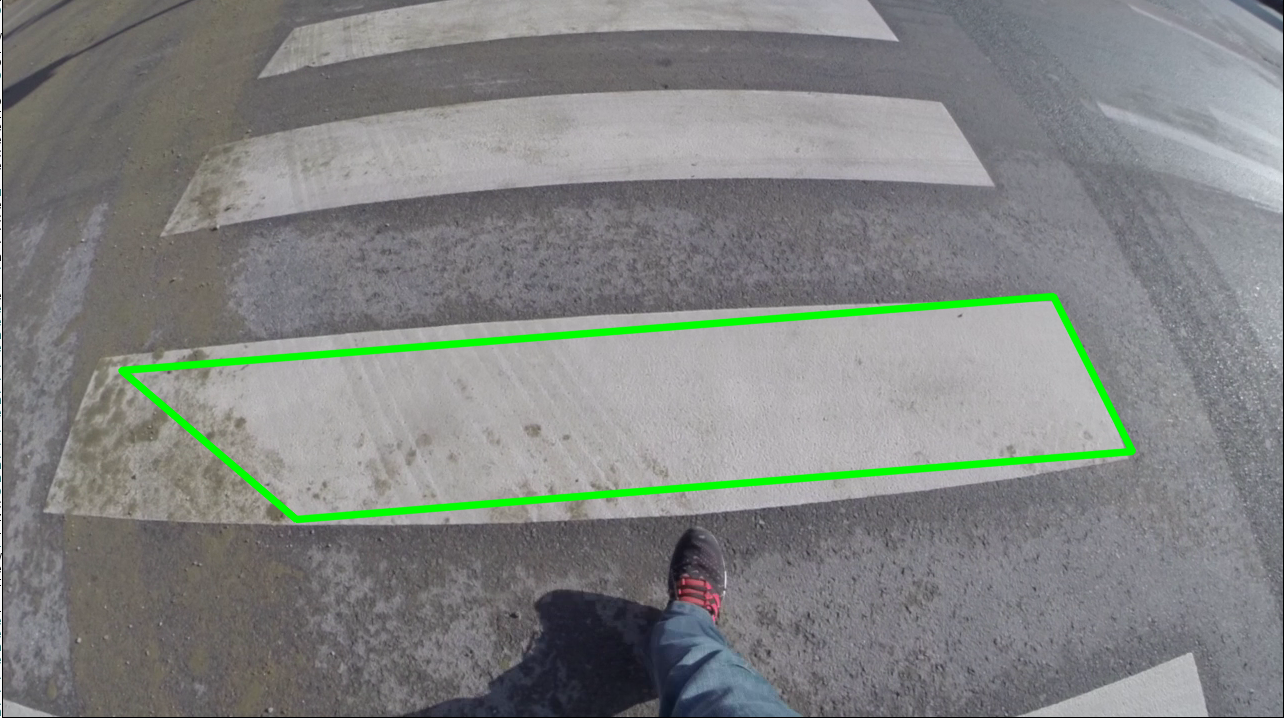
\includegraphics[width=.9\textwidth]{dirtycorner2}
  \caption{\label{dirtycorner2}}
\end{subfigure}
\end{figure}



\clearpage
\clearpage
\subsection{Tiles}
\subsubsection{Idea}
A very obvious feature that can be retrieved from an image is tiles, more specifically how many tiles it contains. This section will explain how a tile can be recognised and how these tiles are used to differentiate between different regions of the path. 
\subsubsection{Recognising tiles}
Shadows, lack of light, dirt  and blurry images are real culprits when it comes down to recognising tiles. To get the best results, the search for rectangles is repeated during multiple iterations. Each iteration applies a different filter to counteract the shadows, dirt and bad image quality. The lack of light is dealt with by repeating the search twice, once on the normal image and once on the image with increased contrast. This repitition is necessary because increasing the contrast on an already bright image reduces the amount of tiles that are be found. The results of the normal and manipulated image are added up and considered the global result for the given image. 
\npar
The search iterations  consist of a few filters that counteract shadows, dirt and bad image quality. Each set of iterations initially converts the received image to a grayscale image. The first iteration applies a Canny\footnote{\url{http://docs.opencv.org/modules/imgproc/doc/feature_detection.html?highlight=canny\#canny}} filter, which is used for finding edges in an image. The aforementioned culprits cause the Canny edges to leave gaps where there shouldn't be. Dilating\footnote{\url{http://docs.opencv.org/modules/imgproc/doc/filtering.html?highlight=dilate\#void dilate(InputArray src, OutputArray dst, InputArray kernel, Point anchor, int iterations, int borderType, const Scalar& borderValue)}} the result from Canny fills up most of these gaps. The Canny and dilate results are shown the figures below.  

\begin{figure}[ht]
\centering
\begin{subfigure}{.5\textwidth}
  \centering
  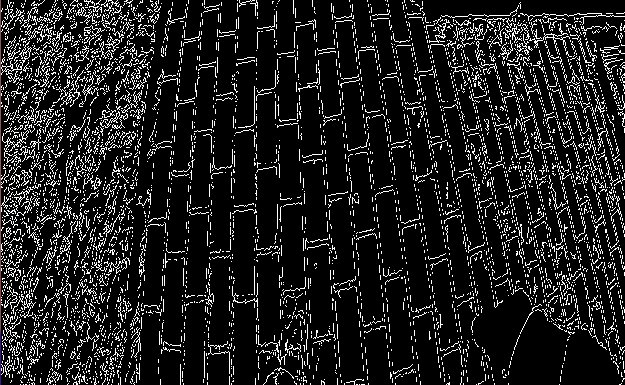
\includegraphics[width=.9\textwidth]{canny}
  \caption{Canny filter\label{canny}}
\end{subfigure}%
\begin{subfigure}{.5\textwidth}
  \centering
  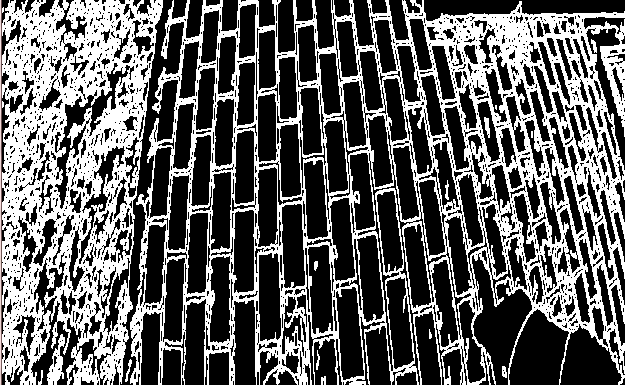
\includegraphics[width=.9\textwidth]{dilate}
  \caption{Dilate\label{dilate}}
\end{subfigure}
\caption{Canny and dilate\label{canny_dilate}}
\end{figure}

The result after dilate appears near perfect, which begs the question why any other filter is required. The answer is simple: Canny reacts very poorly to dirt. As an example consider the left side of the images. This side consists of grass, which is recognised by Canny is a spaghetti of edges. If there was a tile in there, it would be heavily distorted by this grass. The same applies to dirt on a tile. The reason why Canny is used, is because it is not affected by tiles with a gradient shading, which is the downfall of the second filter.
\npar
The remaining iterations apply the same type of filter with a different threshold on each iteration. The pixels of the initial grayscale image with a whiteness intensity above the threshold are copied into a new image. Because tiles are separated by dark grooves, this new image will only contain the tiles. Or rather, this is the goal. Multiple thresholds are required to deal with more or less sunlight making the tiles brighter or darker. Similar to the Canny result, the lines contouring the tiles may not appropriately connect. Erode\footnote{\url{http://docs.opencv.org/modules/imgproc/doc/filtering.html?highlight=dilate\#erode}} is used to shrink the tiles a little bit, improving the boundaries around those tiles. The result is shown below.

\begin{figure}[ht]
\centering
\begin{subfigure}{.5\textwidth}
  \centering
  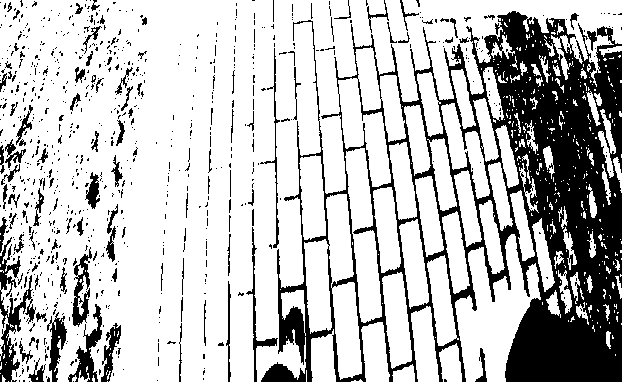
\includegraphics[width=.9\textwidth]{gray}
  \caption{Color intensity thresholding\label{gray}}
\end{subfigure}%
\begin{subfigure}{.5\textwidth}
  \centering
  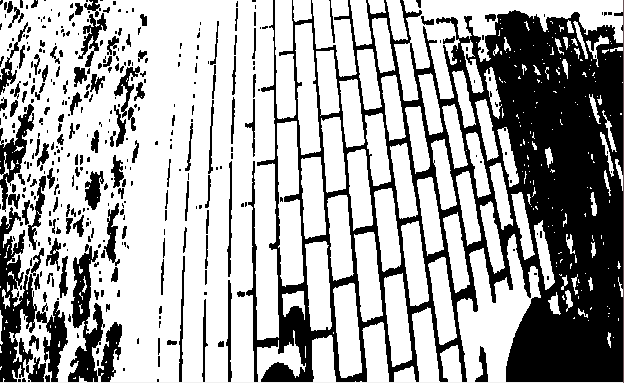
\includegraphics[width=.9\textwidth]{erode}
  \caption{Erode\label{erode}}
\end{subfigure}
\caption{Thresholding and erode\label{gray_erode}}
\end{figure}

\npar
Each filter results in a bunch of contours around the existing tiles. These contours can be retreived with the findContours\footnote{\url{http://docs.opencv.org/modules/imgproc/doc/structural_analysis_and_shape_descriptors.html?highlight=findcontours\#findcontours}} function. This will return every contour found in the image, not just the ones belonging to the tiles. Extracting the useful contours is done in three steps:
\begin{enumerate}
\item{approxPolyDP\footnote{\url{http://docs.opencv.org/modules/imgproc/doc/structural_analysis_and_shape_descriptors.html\#approxpolydp}} is used to approximate the contours with a polygonal.}
\item{Tile contours should have 4 vertices, so every approximated contour that doesn't match this constraint is dropped.}
\item{A tile is a rectangle, meaning its corners should be at a 90 degree angle. Calculating this angle happens through simple math, using the following formula: $v \cdot w = ||v|| * ||w|| cos q$. Every contour that has corners with a cosine greater than $0.3$ is dropped. Note that $0.3$ is chosen as a margin of error, allowing slightly less than perfect rectangles to be accepted. }
\end{enumerate}

\subsubsection{Using tile sizes}
Finding tiles as described above, yields every rectangle ranging from only a few pixels to a square the size of the frame itself. The next step is filtering out unwanted sizes and grouping them into sizes that match certain real tile sizes. The size groups are chosen as following:
\begin{enumerate}
\item{Small tiles: 801 to 4500 pixels}
\item{Medium tiles: 4501 to 19000 pixels}
\item{Large tiles: 19000 to 100000 pixels}
\end{enumerate}
Finding these sizes has been done through trail and error. They have proven to be the best boundaries between the tile sizes found in the given video fragments.
\subsubsection{Setting the boundaries of regions}
Initially, finding proper boundaries for certain regions based on tile sizes proved to be problematic. A tile further ahead appears smaller than it really is, clouding the results with wrong tile sizes. One option could be to manipulate the perspective, turning the image in a top down view. This method however is rather difficult and could potentially distort the boundaries of certain tiles even more. A second approach was used: only use the bottom half of the image.  This approach is quite logical, only take the tiles into account that the person is on right now. Tiles in the distant can be quite irrelivant and can, due to minor detours, have nothing to do with the actual route. The result for first video fragment, the path from the university campus to the train station, is shown in Figure \ref{grafiek_tegelgroottes}.

\begin{figure}[ht]
\centering
  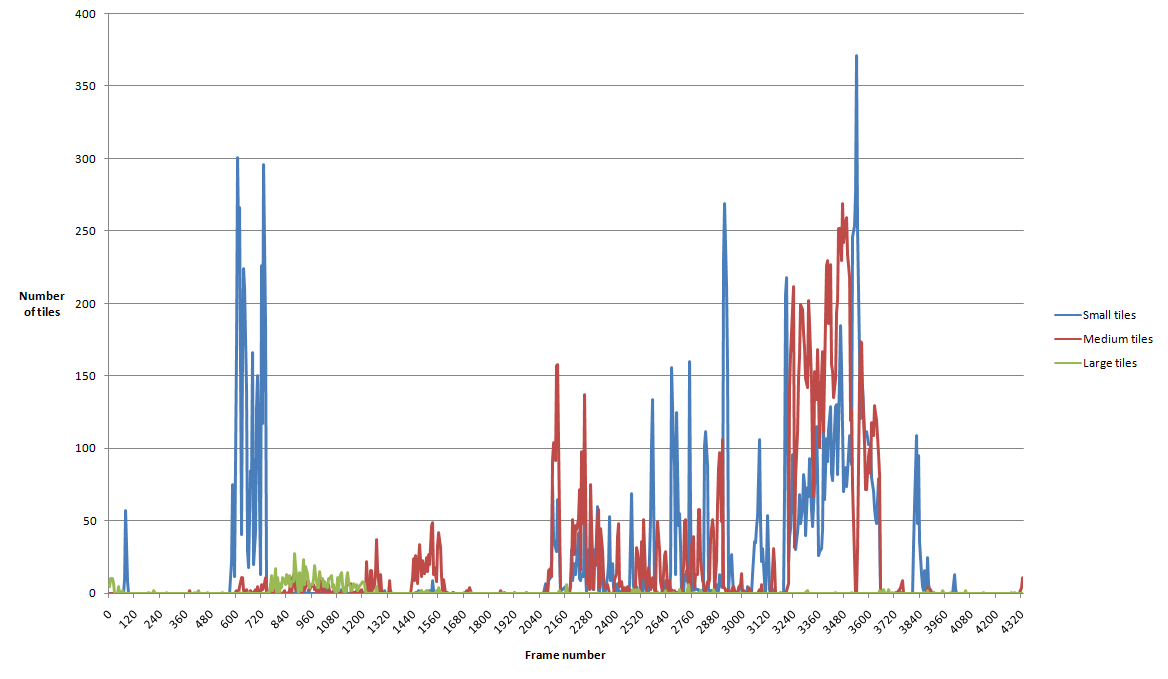
\includegraphics[width=1.1\textwidth]{grafiek_tegelgroottes}
  \caption{Tile count for the first video fragment\label{grafiek_tegelgroottes}}
\end{figure}
The first half of the graph above marks very distinct regions based on the absence or presence of certain tile sizes. The second half is not as fortunate. The Sint-Denijslaan consists of frequent alterations between small and medium tiles, making it difficult to mark large enough regions with a common tile size. Near the end the medium tiles see a significant increase in number. Unfortunately this cannot be used to mark a new region, because there are too many factors that can influence the number of tiles recognised. The result would be too unreliable, especially considering this region lies immediately next to its counterpart with lower, but still significant numbers. For this reason, the boundary leading up to its neighbouring region would have to be be very clear.  

\subsubsection{Conclusion}
Using tile sizes as a feature is definitly an option. It is perfectly suited for giving a raw estimation of where the user is located. This estimation can then be refined by using additional features.
\clearpage

\subsection{Yellow border}
\subsubsection{Idea}
As there are a lot of zones where tiles cannot be recognized, there is still need for extra features. To recognize extra zones, a feature was implemented to detect yellow items. This can be used in combination with other features, like grass, to determine in what zone the person is at that given moment. 

\subsubsection{Finding the color yellow}

To find the color yellow, the image is converted from BGR to HSV. After the image is converted, the colors that lie in a range of HSV values are kept, the others are thrown away. A binairy image is created using the inRange function. The range that is used is (20, 55, 25) - (24, 255, 210) with (H, S, V) respectively. This range is used to detect yellow items, but also to limit the reflection of the bright yellow sunlight. 

\subsubsection{Using the yellow color}
By using the yellow color in combination with other features, it is possible to recognize zones which couldn't be recognized without the yellow color. However, this is not sufficient to be certain that the correct zone is identified. In order to solve this problem, an extra feature was added.

\subsubsection{Detecting yellow rectangles}
By detecting yellow rectangles, the zone with yellow borders can be identified better. To implement this feature, detecting yellow is used as a base. A problem with this, is the yellow sunlight which causes to reflect bright yellow on some items. To solve this a threshold was added to filter out bright items before the yellow color gets detected. A second problem that occured, is that not enough yellow was returned. The range in which yellow was searched had to be set broader. The range got changed into ((20, 40, 40) - (23, 255, 255). Only thing left is to detect rectangles. But this is the same as detecting squares, so the same code could be used to detect rectangles in this case. The only difference is the source image, the image used here is an image of only yellow items. 
\subsection{Contrast}

While the tile detection algorithm was working pretty good, there were some regions in which the tiles are visible with the naked eye, but could not be detected. To resolve this, some code was added to adjust the contrast of the images. 

\subsubsection{Adjusting contrast}

To adjust the contrast of an image, a new image has to be created where a specific formula is used for every pixel. To complete this task, every pixel of the original image must be accessed. Since the image is in BGR, three values must be changed per pixel. To change the contrast, each of the three values of every pixel must be multiplicated with a variable, which will be noted as \textalpha. \textalpha  \ lies in a range of 1.0-3.0. Since this variable is a float, the result of this multiplication may not be an integer. To solve this problem this result must be saturated. The formula used to adjust the contrast can be noted down as \textalpha \  $ \cdot $ p(i, j) where p is the pixel located on column i and row j.

\subsubsection{Brightness}

With a slight modification to the formula, it is also possible to adjust the brightness of an image. Altough this was not used for this application, it is still useful to note this down. The formula to adjust the contrast and brightness of an image is \textalpha \  $ \cdot $ p(i, j) + \textbeta. \textbeta is an integer which lies in the range 0-100.


%segmentatie => uitleggen welke zone gebruikt worden en welke features we daaruit willen herkennen
\clearpage
\section{Segmentation}

Using the features discussed in the previous section it was possible to divide the given route into multiple zones as shown in Figure \ref{zones}.
\mijnfiguur{width=0.5\textwidth}{zones}{A table overview of the zones and their features}

The table is transformed into a decision tree. Following the tree, left for yes and right for no, each frame can be classified with it corresponding zone, see Figure \ref{zones}.

\mijnfiguur{width=0.5\textwidth}{tree1}{Left part of the decision tree}
\mijnfiguur{width=0.5\textwidth}{tree2}{Right part of the decision tree}
\clearpage
Later a distinction was added to zone 10. Splitting it in two zones: zone 10, the zebra crossing as discussed in section \ref{zebrasection} and zone 11: the station. However since the zebra detection doesn't work properly, zone 10 is ignored. The division was done since the difference between a zebra crossing at a busy street from a busy station is very important for a blind person.


%\clearpage %mss wat overdreven asl er ma 5 zinnen staan op vorige pagina
\section{Conclusion}
The use of image processing is not always reliable due to changes in the surrounding e.g. roadworks, more light, less light, seasons that change the color the vegetation. A solution can be found for most of these problems, but that requires a lot of time
\npar
Keeping in mind that this system is only 12 weeks in development, some promissing results were found.
Most zones are identified and since the ultimate goal is a combination of image processing with a GPS, some false positives are allowed.
\npar
However this system is far from complete, there are still problems that require a solution. For instance when the light intensity is low, tiles aren't recognized. When shadow of the blind person covers the rectangles of a pedestrian crossing, the crossing isn't recognized.
\npar
A more complex approach is needed to solve these problems. To make this system more reliable in different seasons and conditions, more training is needed.

%backmatter
%
% ---- Bibliography ----
%
\clearpage
\begin{thebibliography}{8}
%
\bibitem {Burges}
Burges, Christopher J.C.:
A Tutorial on Support Vector Machines for Pattern
Recognition (1998)

\bibitem {Hears}
Hears, M. A.:
Support vector machines (1998)


\bibitem {Boswell}
Boswell, D:
Introduction to Support Vector Machines (2002)

\bibitem {Jinwei}
Jinwei G.:
An Introduction of Support Vector Machine (2008)

\bibitem {Dahlkamp}
Dahlkamp H. et al.:
Self-supervised Monocular Road Detection in
Desert Terrain (2005)

\bibitem{Nguyen}
Nguyen T. S.: Automatic detection and classification on roead pavedment usin anisotropy measure (2009)

\bibitem{BGR}
Shipman J. W.: The color wheel and the RGB color model, \url{http://infohost.nmt.edu/tcc/help/pubs/colortheory/web/color-wheel.html}, 2012

\bibitem{HSV}
Shipman J. W.: The hue-saturation-value (HSV) color model, \url{http://infohost.nmt.edu/tcc/help/pubs/colortheory/web/hsv.html}, 2012
\end{thebibliography}

\clearpage


\end{document}